\documentclass[tikz,border=2pt]{standalone}
\usepackage{amsmath,amssymb}
\usepackage{pgfplots}
\pgfplotsset{compat=1.18}
\usetikzlibrary{arrows.meta}
\begin{document}
% M/M/1 queue: E[L] = rho/(1-rho) against the load rho on [0, 0.95]; points at rho = 0.4 (2/3),
% 0.8 (4) and 0.95 (19, Riley's single oven); no stationary distribution for rho >= 1.
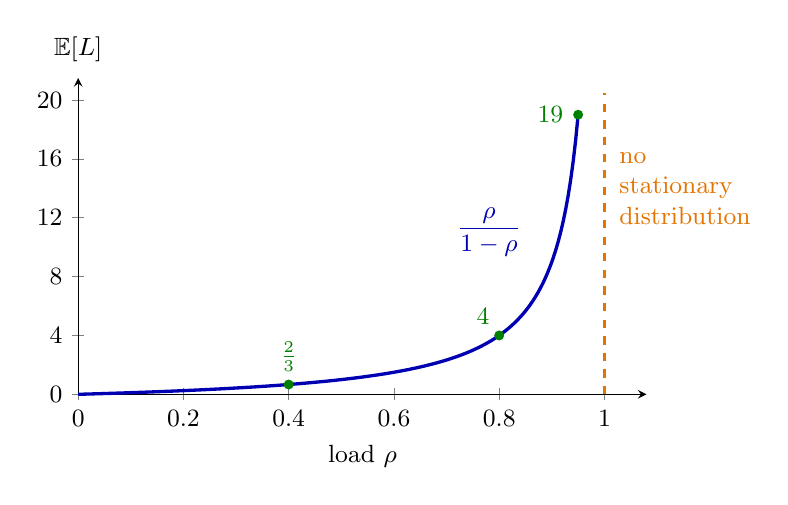
\begin{tikzpicture}[font=\small, >={Latex[length=2mm]}]
  \begin{axis}[
    axis lines=left, xmin=0, xmax=1.08, ymin=0, ymax=21.5,
    xtick={0,0.2,0.4,0.6,0.8,1}, ytick={0,4,8,12,16,20},
    xlabel={load $\rho$}, ylabel={$\mathbb{E}[L]$},
    ylabel style={rotate=-90, anchor=south, at={(axis description cs:0,1.02)}},
    width=8.8cm, height=5.6cm, clip=false]
    \draw[orange!90!black, thick, dashed] (axis cs:1,0) -- (axis cs:1,20.5);
    \node[orange!90!black, anchor=west, align=left] at (axis cs:1.01,14) {no\\stationary\\distribution};
    \addplot[blue!70!black, very thick, domain=0:0.95, samples=200] {x/(1-x)};
    \node[blue!70!black, anchor=east] at (axis cs:0.86,11) {$\dfrac{\rho}{1-\rho}$};
    \fill[green!50!black] (axis cs:0.4,0.6667) circle (1.8pt);
    \fill[green!50!black] (axis cs:0.8,4) circle (1.8pt);
    \fill[green!50!black] (axis cs:0.95,19) circle (1.8pt);
    \node[green!50!black, anchor=south] at (axis cs:0.4,0.9) {$\tfrac{2}{3}$};
    \node[green!50!black, anchor=south east] at (axis cs:0.8,4.1) {$4$};
    \node[green!50!black, anchor=east] at (axis cs:0.94,19) {$19$};
  \end{axis}
\end{tikzpicture}
\end{document}
